\UseRawInputEncoding
\documentclass[12pt]{beamer}
\usecolortheme[named=red]{structure}

\usepackage[T1]{fontenc}
\usepackage[utf8]{inputenc}
\usepackage{lmodern}

\def\magyarOptions{defaults=hu-min}
\usepackage[magyar]{babel}
\usepackage[autostyle]{csquotes}
\DeclareQuoteStyle{magyar}{,,}{''}{>>}{<<}

%\usetheme{CambridgeUs}
\usepackage{epstopdf}
\usepackage{graphicx}
\usepackage{wrapfig}
\usepackage{amsmath}
\usecolortheme{beaver}
\usepackage{siunitx}
\hypersetup{unicode=true}

\setbeamertemplate{enumerate items}[circle]
\setbeamertemplate{itemize items}[circle]
 
%Information to be included in the title page:
\title[Doktori téma]{Stochastic properties of\\dislocation motion and rearrangement\\{\small Investigated by cellular automata and experiments}}

\author[Tüzes]{Tüzes Dániel\\\vspace{1em}Témavezetők: Groma István, Ispánovity Péter Dusán\\Advisor: Michael Zaiser}
 
\institute[ELTE Fizika Doktori Iskola] % (optional)
{
  Anyagtudomány és szilárdtestfizika, Fizika Doktori Iskola, ELTE TTK
}

\date{Doktori védés\\2019. május 3.}

\begin{document} 
\frame[plain]{\titlepage}
 
 
\section{Motiváció}
\begin{frame}
\frametitle{Motiváció: deformáció a mikronos tartományban}
\begin{center}
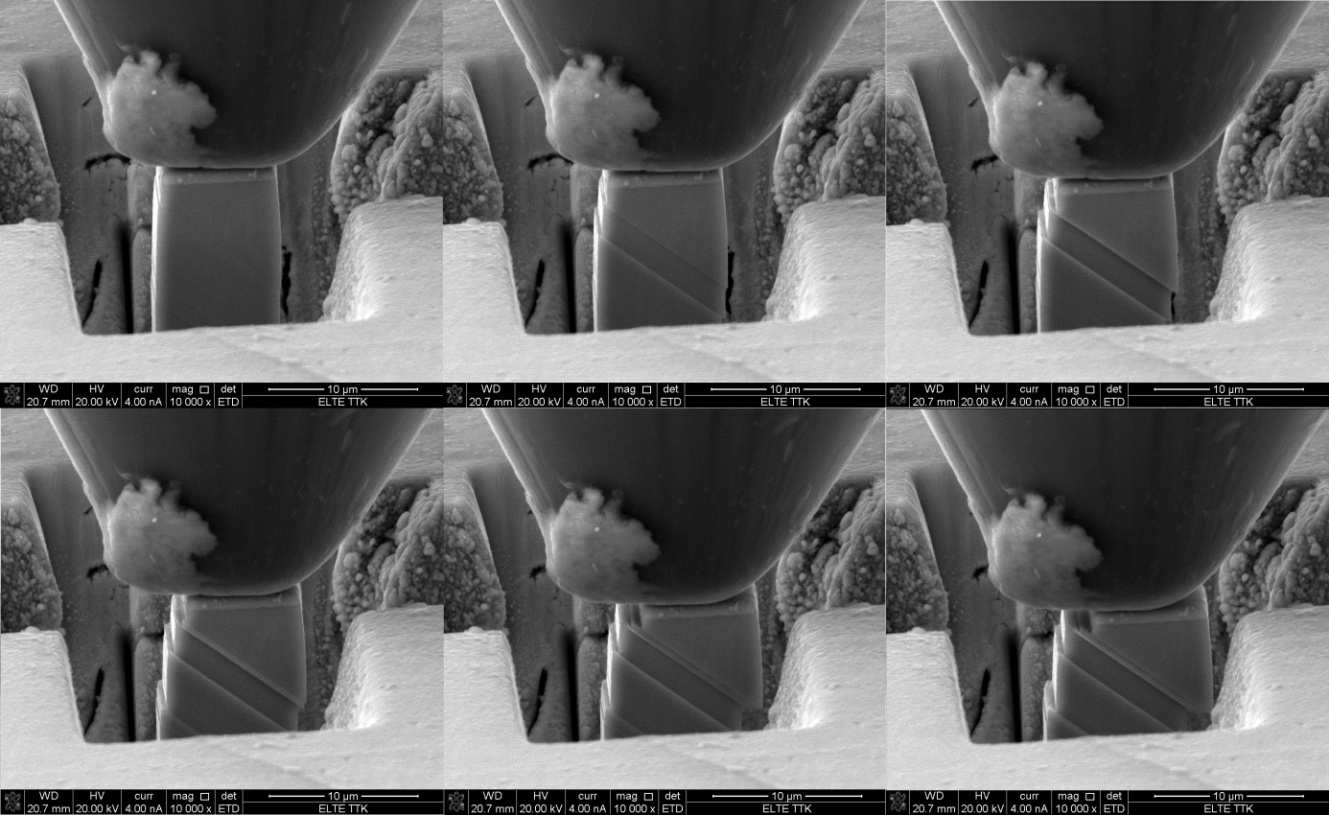
\includegraphics[width=0.8\textwidth]{figs/bazalisZn28840.png} 
\end{center}
Cink egykristály deformációs tesztje\\(\SI{8}{\micro\meter}, egyszeres bazális csúszásra orientált)
\end{frame}

\begin{frame}
\frametitle{Motiváció: diszlokiációk mintázata}

\begin{columns}
\begin{column}{0.5\textwidth}
  \begin{center}
  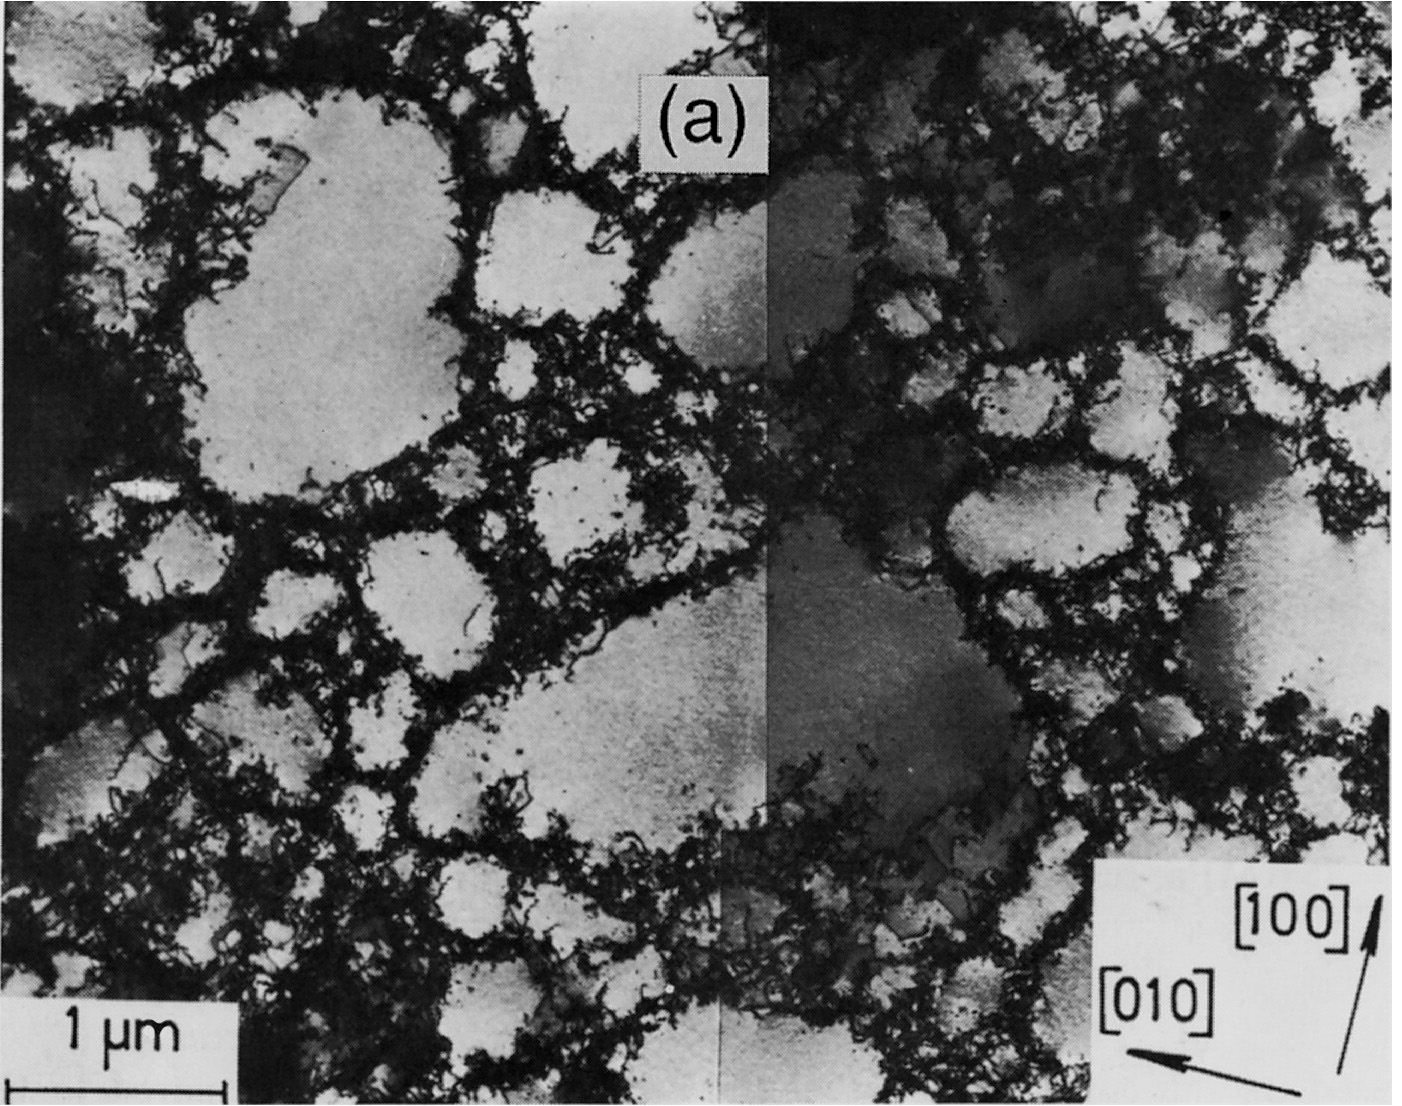
\includegraphics[scale=0.44]{figs/disloc_fractal.jpg}
  \end{center}
  Fraktál-szerkezet, többszörös csúszási rendszerre orientálva (TEM).
\end{column}
\begin{column}{0.5\textwidth}  %%<--- here
  \begin{center}
  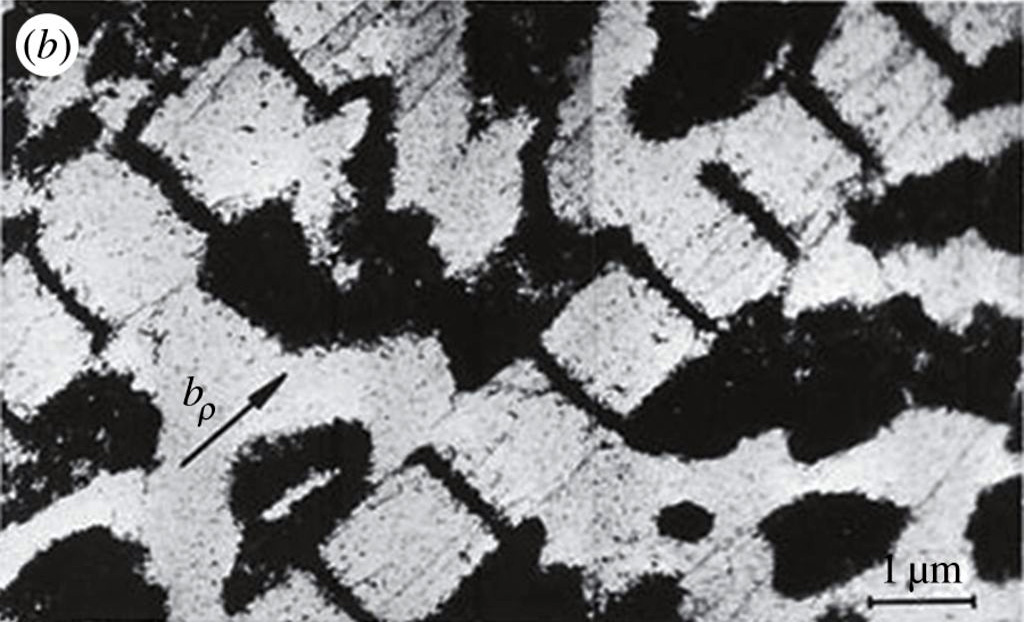
\includegraphics[scale=0.6]{figs/disloc_psb_m.jpg}
  \end{center}
  Lépcsős szerkezetek megjelenése a diszlokáció- mátrixban, fárasztás, PSB megjelenése (TEM).
\end{column}
\end{columns}

\end{frame}

\begin{frame}
\frametitle{Motiváció: modellezési nehézségek}
Diszlokációk modellezése 2D-ban, DDD
  \begin{center}
  \includegraphics[scale=1]{figs/ddd.eps}
  \end{center}
\begin{itemize}
\item hosszú hatótávú kölcsönhatás (memória lokalizáció hiánya)
\item kölcsönhatások száma $\propto N^2$
\item a közeli diszlokációk rontják az időlépést
\end{itemize}
\end{frame}


\begin{frame}
\frametitle{Motiváció: kísérleti vizsgálatok}
\begin{itemize}
\item Nanoindentációs tesztek hatékonyak
\item Akusztikus jelek, vizuális megjelenés
\end{itemize}
\begin{columns}
\begin{column}{0.51\textwidth}
  \begin{center}
  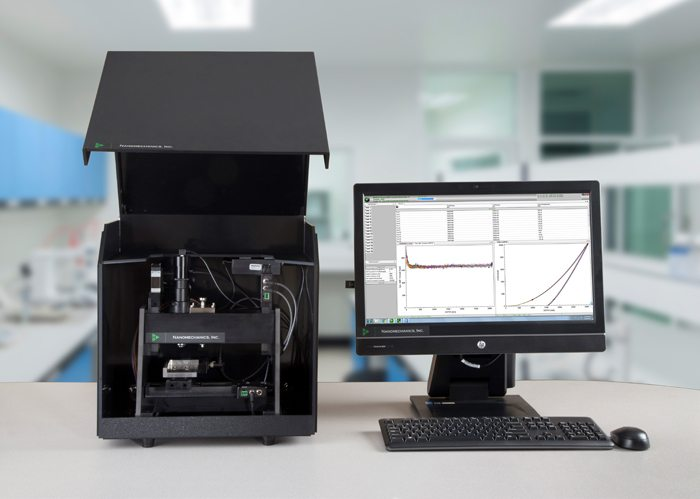
\includegraphics[width=1\textwidth]{figs/newnanopicture.jpg}
  \end{center}
 Kis méretű nanoindenter.
\end{column}
\begin{column}{0.5\textwidth}  %%<--- here
  \begin{center}
  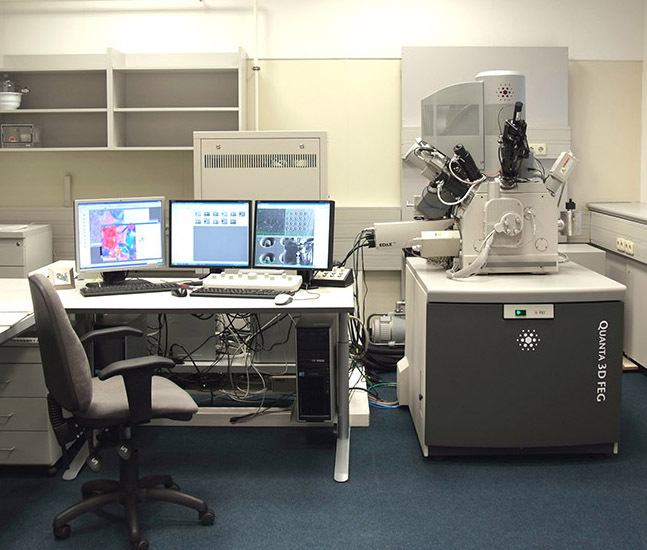
\includegraphics[width=1\textwidth]{figs/SEM-laboratorium.jpg}
  \end{center}
Pásztázó elektronmikroszkóp
\end{column}
\end{columns}
\end{frame}




\section{Elmélet}
\begin{frame}
\centering
\Huge Elmélet\\
\large A numerikus számoláshoz használt modellhez
\end{frame}



\begin{frame}
\frametitle{Térmennyiségek}
\centering\includegraphics<1>[width=0.5\textwidth]{figs/mean_field_DDD.eps}\includegraphics<2>[width=0.5\textwidth]{figs/mean_field_DDD_averaged.eps}\begin{columns}\begin{column}{0.5\textwidth}\includegraphics<3->[width=1\textwidth]{figs/mean_field_kappa_wDDD.eps}\onslide<3->{\\\vspace{-1.5em}\[\kappa  = \left( {{N_ + } - {N_ - }} \right)/T\]}\end{column}\begin{column}{0.5\textwidth}\includegraphics<4->[width=1\textwidth]{figs/mean_field_rho_wDDD.eps}\onslide<4->{\\\vspace{-1.5em}\[\rho  = \left( {{N_ + } + {N_ - }} \right)/T\]}
\end{column}
\end{columns}
\only<1,2>{
\begin{itemize}
\item Diszlokációk egyenkénti koordinátája
\onslide<2>
\item Térmennyiségek valamilyen kiátlagolással
\end{itemize}}
\onslide+<5>\vspace{-0.9em}\begin{itemize}
\item Mennyi részlet veszik el? Mennyi veszhet el?
\item Elég az átlagtér-elmélet? Lavina: igen. Mintázat: nem.
\end{itemize}
\end{frame}


\section{Modellek}
\begin{frame}
\centering
\Huge Modellek \vspace{1em}
\large
\begin{itemize}
\item[{[1]:}] lavinamodellezés
\item[{[2]:}] törési modell
\item[{[3]:}] diszlokáció mintázat
\end{itemize}
\end{frame}



\subsection{SCPM}
\begin{frame}
\frametitle{[1] Mikroszerkezet figyelembe vétele}
\begin{itemize}
\item<1-> $\kappa$ teret megtartjuk, $\rho$ változását elhanyagoljuk
\item<2> bevezetünk helyi folyásfeszültség-értékeket
\item<2> sztochasztikus modell
\end{itemize}

\begin{columns}
\begin{column}{0.51\textwidth}
  \begin{center}
  \includegraphics<1->[width=1\textwidth]{figs/mean_field_kappa.eps}
  \end{center}
\end{column}
\begin{column}{0.5\textwidth}  %%<--- here
  \begin{center}
  \includegraphics<2>[width=1\textwidth]{figs/mean_field_tau.eps}
  \end{center}
\end{column}
\end{columns}

\end{frame}

\begin{frame}
\frametitle{[1] Szimulációs protokoll - inicializáció}
\begin{itemize}
\item külső nyíróerő 0
\item \onslide<2-> $\kappa$ 0 (fehér); deformáció 0 (0)
\item<3> \onslide<3> A helyi folyásfeszültség korrelálatlan, random változó
\end{itemize}

\begin{columns}
\begin{column}{0.5\textwidth}
  \begin{center} \onslide<2->
  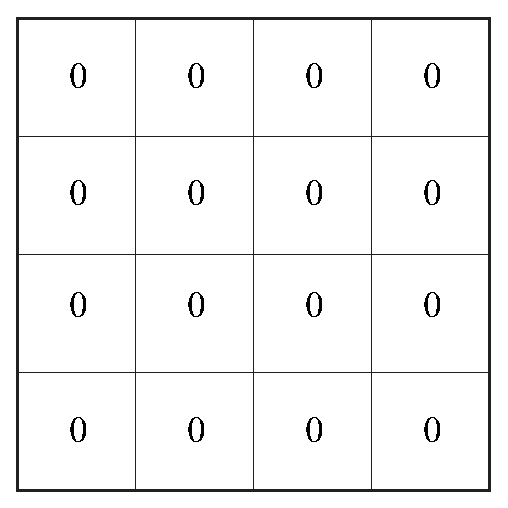
\includegraphics[width=0.91\textwidth]{figs/mean_field_empty.eps}
  \end{center}
\end{column}
\begin{column}{0.5\textwidth}  %%<--- here
  \begin{center} \onslide<3>
  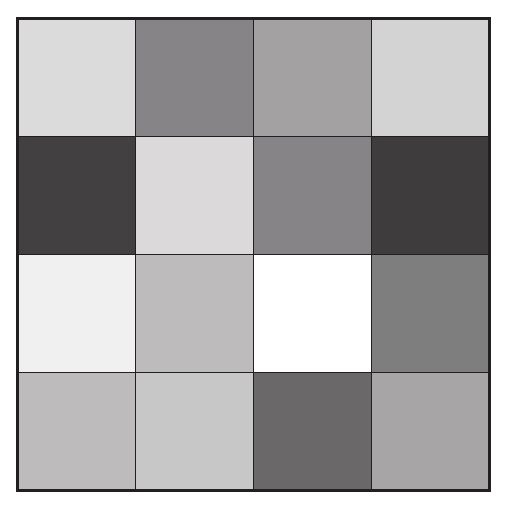
\includegraphics[width=0.91\textwidth]{figs/mean_field_tau.eps}
  \end{center}
\end{column}
\end{columns}

\end{frame}


\begin{frame}
\frametitle{[1] Szimulációs protokoll - lavina kezdet}
\begin{itemize}
\item<1-> A nyírófeszültséget növeljük, amíg
\item<2-> a leggyengébb cella megfolyik
\item<3-> új deformáció, új $\kappa$, új folyásfeszültség
\end{itemize}

\begin{columns}
\begin{column}{0.5\textwidth}\begin{center}\includegraphics<1,2>[width=0.91\textwidth]{figs/mean_field_empty.eps}\includegraphics<3>[width=0.91\textwidth]{figs/mean_field_kappa_def1.eps}\end{center}\end{column}
\begin{column}{0.5\textwidth}\begin{center}\includegraphics<1>[width=0.91\textwidth]{figs/mean_field_tau.eps}\includegraphics<2>[width=0.91\textwidth]{figs/mean_field_tau_star.eps}\includegraphics<3>[width=0.91\textwidth]{figs/mean_field_tau_def1.eps}\end{center}\end{column}
\end{columns}

\end{frame}



\begin{frame}
\frametitle{[1] Szimulációs protokoll - lavina vég}
\begin{itemize}
\item<1-> A nyírófeszültséget állandó értéken tartjuk
\item<2-> a külső nyíróerő + $\kappa$ generálta tér megfolyat új cellát?
\item<3> új deformáció, új $\kappa$, új folyásfeszültség
\end{itemize}

\begin{columns}
\begin{column}{0.5\textwidth}
  \begin{center}\includegraphics<1,2>[width=0.91\textwidth]{figs/mean_field_kappa_def1.eps} \includegraphics<3>[width=0.91\textwidth]{figs/mean_field_kappa_def2.eps}\end{center}
\end{column}
\begin{column}{0.5\textwidth}  %%<--- here
  \begin{center}\includegraphics<1>[width=0.91\textwidth]{figs/mean_field_tau_def1.eps}\includegraphics<2>[width=0.91\textwidth]{figs/mean_field_tau_def1_star.eps}\includegraphics<3>[width=0.91\textwidth]{figs/mean_field_tau_def2.eps}\end{center}
\end{column}
\end{columns}

\end{frame}



\begin{frame}
\frametitle{[1] Felparaméterezés: mik a paraméterek?}
Mik a modell jellemző paraméterei?

\begin{enumerate}
\item A folyásfeszültség eloszlása (2 paraméter)
\item Az elemi deformáció nagysága (1 paraméter)
\end{enumerate}

Kalibráljuk ezeket DDD szimulációk eredményei alapján!

\end{frame}



\begin{frame}
\frametitle{[1] Felparaméterezés: mi az eloszlásfüggvény?}
\begin{enumerate}
\item
A folyásfeszültségek egy Weibull-eloszlást követnek,
\[P\left( x \right) = C \cdot {x^{\beta  - 1}} \cdot {e^{ - {{\left( {x/{x_{{\text{sc}}}}} \right)}^\beta }}},\]
\begin{columns}
\begin{column}{0.15\textwidth} \end{column}
\begin{column}{0.31\textwidth}
amelyben
\begin{itemize}
\item $C$:\\normálási faktor
\item $\beta$:\\alakparaméter
\item $x_{\rm{sc}}$:\\skálaparaméter
\vspace{3em}
\end{itemize}
\end{column}
\begin{column}{0.6	\textwidth}
\centering
\includegraphics[width=1\textwidth]{figs/weibull.pdf}
\end{column}
\end{columns}
\end{enumerate}

\end{frame}



\begin{frame}
\frametitle{[1] Felparaméterezés: mi deformációs lépés?}
\begin{enumerate}
\setcounter{enumi}{1}
\item
Az elemi deformáció keltette feszültség és az eloszlás átlagának aránya:\\
\end{enumerate}

\centering
\includegraphics[width=0.8\textwidth]{figs/stress_strain_comparison.pdf}
\end{frame}


\begin{frame}
\frametitle{[1] Eredmények}
Az SCP modell 2 paraméterét DDD-ből illesztve:
\begin{enumerate}
\item helyes lavina - külső feszültség kapcsolata
\item feszültség-deformációs görbe
\end{enumerate}
Számos további hasonlóság:
\begin{itemize}
\item adott deformációnál a feszültségek eloszlása
\item az egymást követő lavinákhoz tartozó külső feszültségek szórása és deformációk eloszlása
\item paraméterek rendszerméretfüggése
\end{itemize}
Az SCPM előnye, hogy nem számítás-igényes.
\end{frame}


\subsection{SCPM kiegészítve}
\begin{frame}
\frametitle{[2] Egy eltérő alkalmazás}
Cél: olyan anyagok törésének vizsgálata, amelyek
\begin{itemize}
\item \pause Makroszkopikusan homogének, mikroszkópikusan rendezetlenek
\item Alakítási lágyulást szenvednek
\item Törésük visszavezethető a deformáció lokalizációjára
\end{itemize}
Példa: fémüvegek, fémhabok.\\
Modell módosítása, kiegészítése:
\begin{itemize}
\item \pause Alakítási lágyulás bevezetése: \[\tau _{i,j}^{{\text{th}}} \cdot \left( {1 - \frac{{\gamma _{i,j}^{{\text{pl}}}}}{{16}}} \right) \mapsto \tau _{i,j}^{{\text{th}}}\]
\item Törés definiálása: ha van olyan cella, amelyre \[\gamma_{i,j}^{{\rm{pl}}} = 16.\]
\item Deformáció kontrollált szimuláció
\end{itemize}
\end{frame}

\begin{frame}
\frametitle{[2] Mi a rendezetlenség?}
\[P\left( x \right) = C \cdot {x^{\beta  - 1}} \cdot {e^{ - {{\left( {x/{x_{{\text{sc}}}}} \right)}^\beta }}},\]
$\beta$ csökkentésével nő a rendezetlenség.
\centering
\includegraphics[width=0.72\textwidth]{figs/weibull.pdf}

\end{frame}


\begin{frame}
\frametitle{[2] Hogyan hat a rendezetlenség?}
$\beta$ csökkenésével szívósabbá válik az anyag.
\centering
\includegraphics[width=0.65\textwidth]{figs/linS_1_4_1000-1512_s_tsc_DsG.pdf}


\end{frame}


\begin{frame}
\frametitle{[2] Mi okozza a megnövekedett szívósságot?}
\centering
\includegraphics[width=0.72\textwidth]{figs/loc-strain-maps-1-4-highest-stress-and-strain_mod.pdf}
\\
A deformáció a nagy rendezetlenségű esetben\\kevésbé lokalizálódik.
\end{frame}



\begin{frame}
\frametitle{[2] A rendezetlenség szerepe a törésben}
\centering
Egyszerűsített kép:
\begin{itemize}
\item A deformáció eleinte homogén,
\item majd véges vastagságú rétegben koncentrálódik
\end{itemize}
\includegraphics[width=0.65\textwidth]{figs/mean_strain_to_failure.pdf}
\end{frame}

\begin{frame}
\frametitle{[2] Eredmények}
\begin{itemize}
\item Fémüvegek és fémhabok intuitív modellje
\item Következetes eredmény: a belső rendezetlenségű anyagban a rendezetlenséget növelni jó
\end{itemize}
A modell előnye: gyorsabb az MD-nél
\end{frame}




\subsection{Mintázaképződés}
\begin{frame}
\frametitle{[3] Kétrészecske-sűrűség figyelembe vétele}
\[{\rho _2}\left( {{{\mathbf{r}}_1},{{\mathbf{r}}_2}} \right)\onslide<1>{?}\onslide<2->{~} = \rho \left( {{{\mathbf{r}}_1}} \right)\rho \left( {{{\mathbf{r}}_2}} \right)\onslide<2->\left( {1 + d\left( {{{\mathbf{r}}_1},{{\mathbf{r}}_2}} \right)} \right)\]
\begin{itemize}
\item Lokális sűrűség közelítés (LDA)
\item A feszültségek kicsik, lassú deformáció
\end{itemize}

\pause
A mozgásegyenletben új tagok jelennek meg:
\pause
\begin{itemize}
\item $ + A \cdot {\partial _x}\rho $ (diffusion stress),
\item $ + D \cdot {\partial _x}\kappa $ (back stress),
\item módosított: $\propto \sqrt{ \rho } $
\end{itemize}

Egy ilyen modellben van mintázatképződés!
\end{frame}


\begin{frame}
\frametitle{[3] Hogyan fejlődik $\kappa$?}
\centering
$\gamma$: plasztikus deformáció
\includegraphics[width=0.8\textwidth]{figs/kappa_direct_space_AD=0_1_small_dislocatom.pdf}
\end{frame}



\begin{frame}
\frametitle{A hullámhossz függése a paraméterektől}
\centering
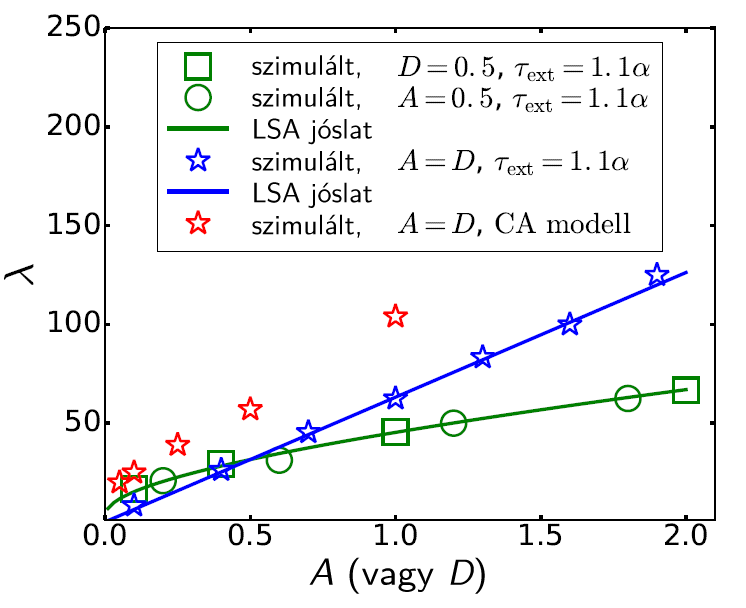
\includegraphics[scale=0.3]{figs/fitted.png} 
\end{frame}


\begin{frame}
\frametitle{Eredmények}
\begin{itemize}
\item Modellezni tudtam a kristályos anyagokban a diszlokációmintázat-képződést
\item A lineáris stabilitáselemzéssel összhangban van az eredmény
\item Vizsgálhatóvá váltak a dl. mintázatok a lineráis közelítésen túl
\item A mintázatok robosztusokak: lényegesen eltérő implementációk is hasonló eredményt adnak
\end{itemize}
\end{frame}



\begin{frame}
\centering
\Huge Kísérlet
\end{frame}

\begin{frame}
\frametitle{[4] Nanoindenter erőmérő cellája}
\centering
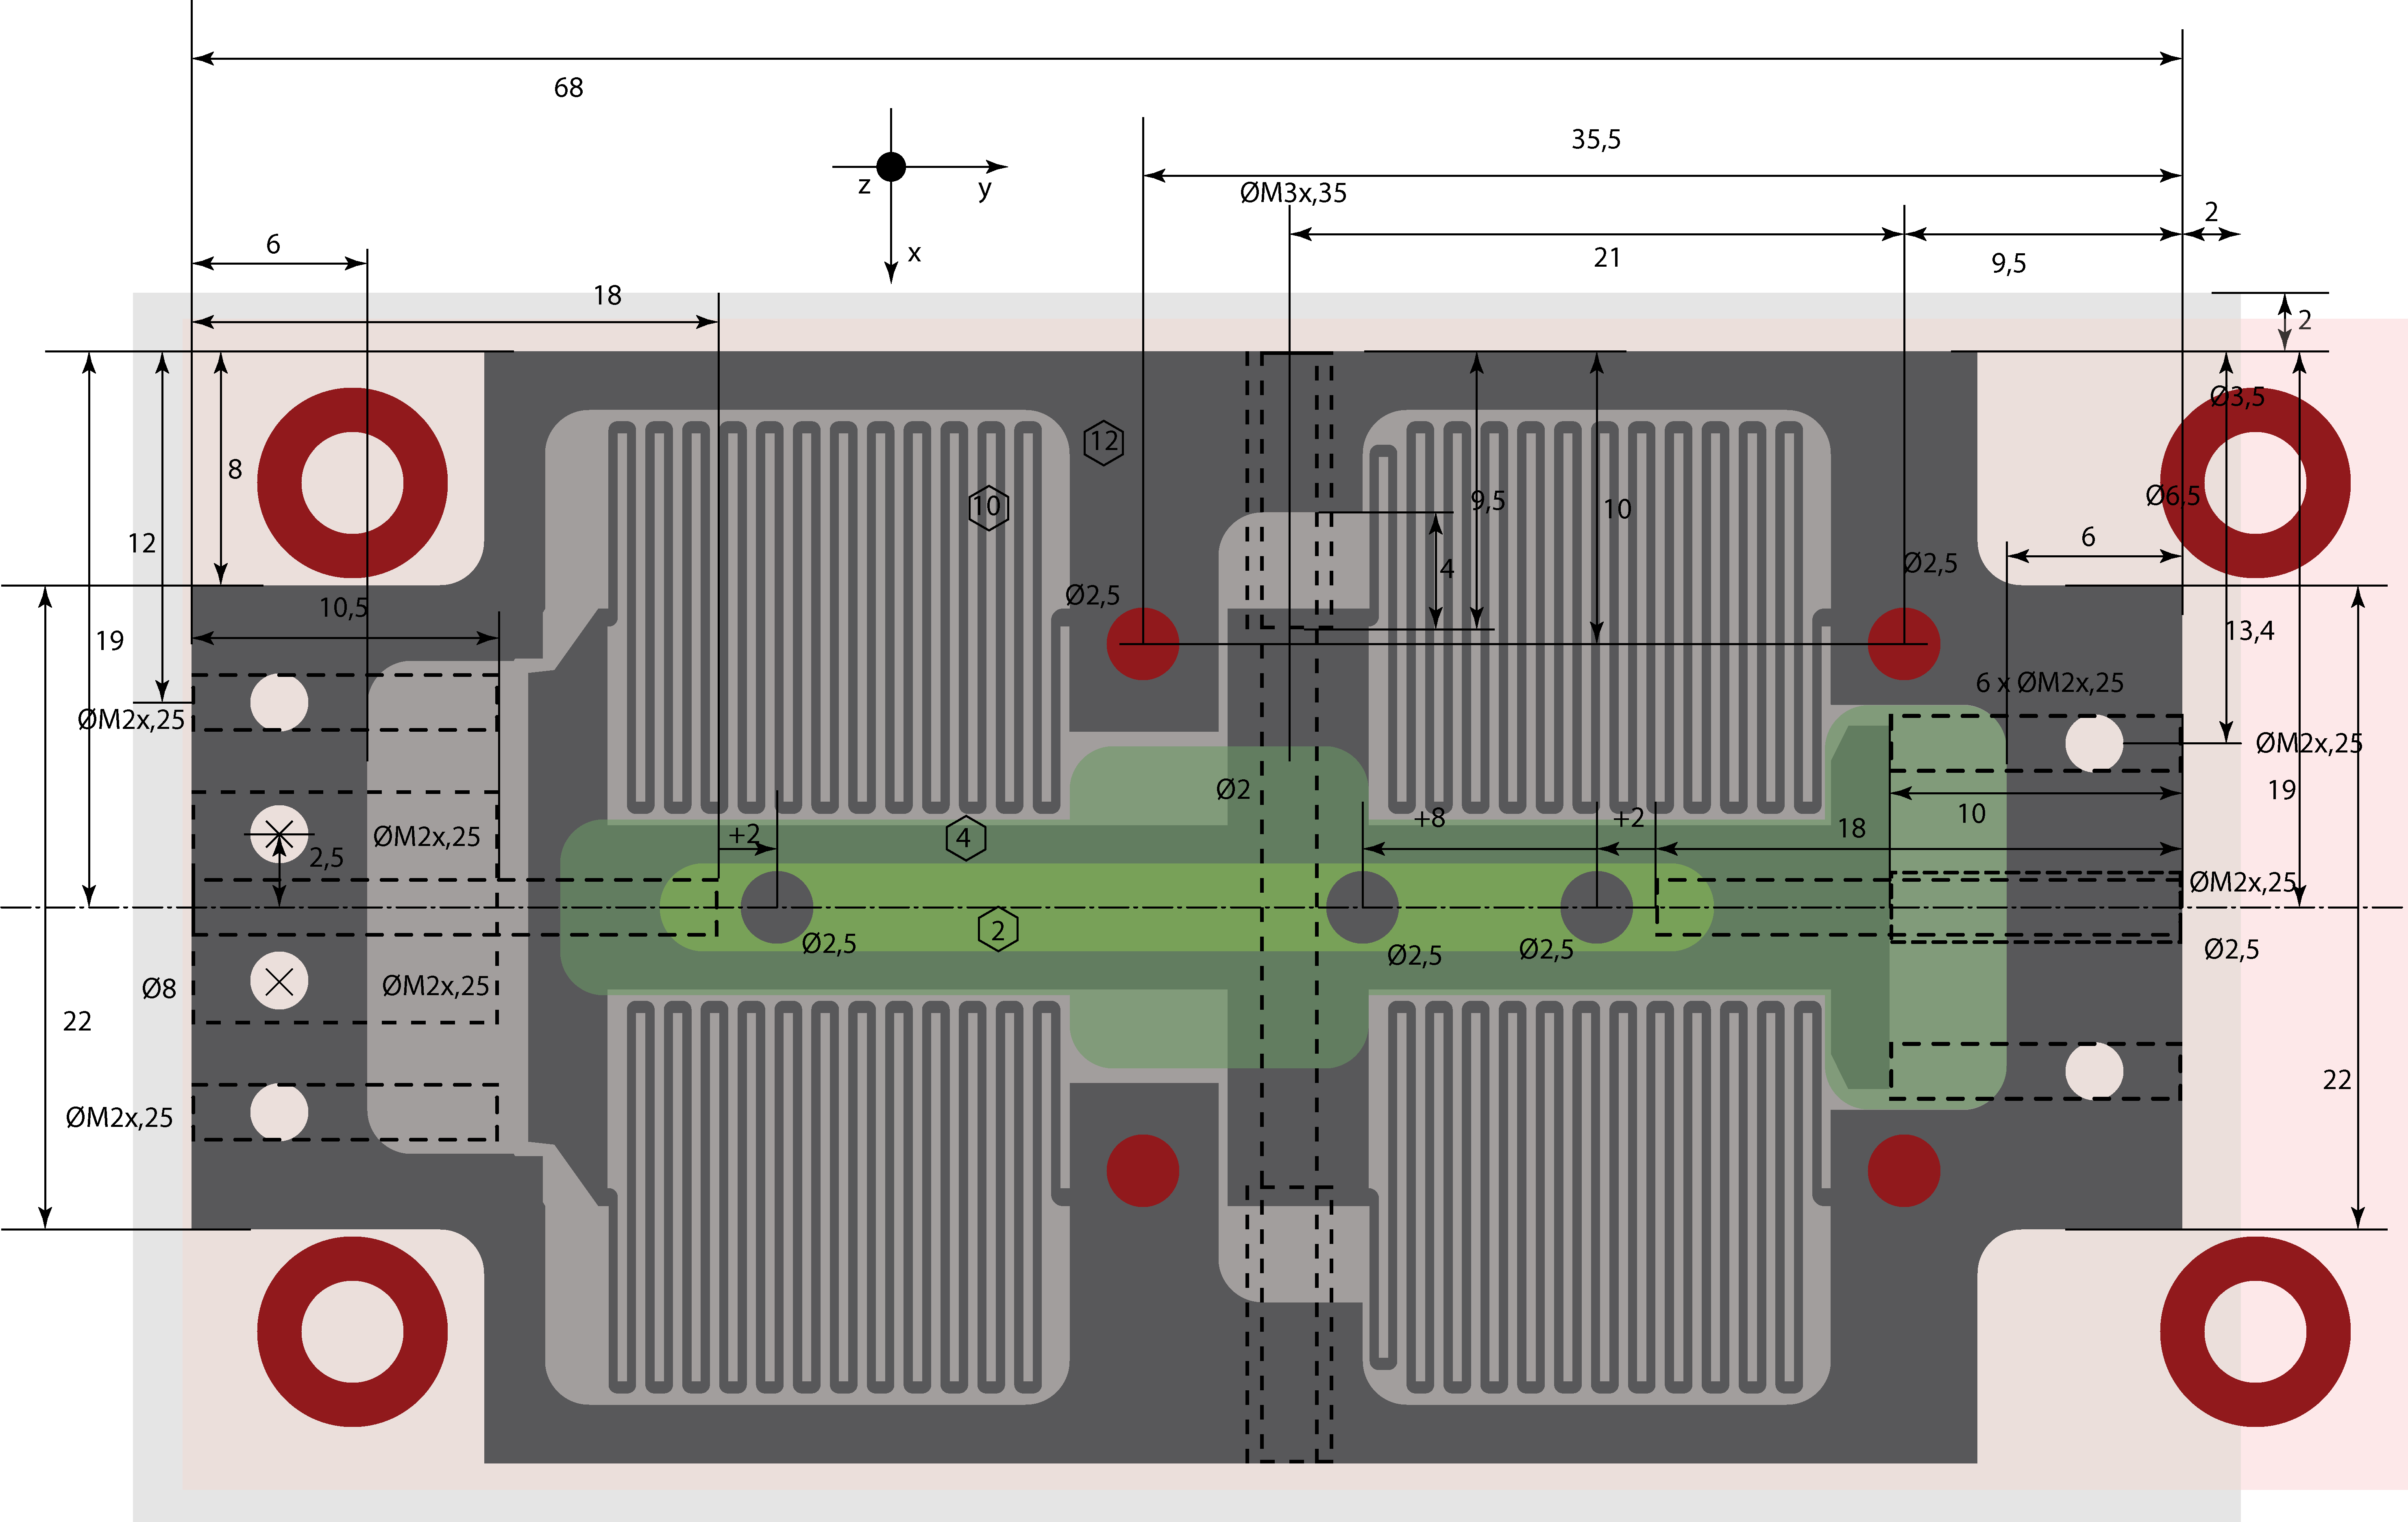
\includegraphics[width=1\textwidth]{figs/nagy_nanoindenter_korrig_forgatva.png} 
\end{frame}


\begin{frame}
\frametitle{[4] Mérési összeállítás}
\centering
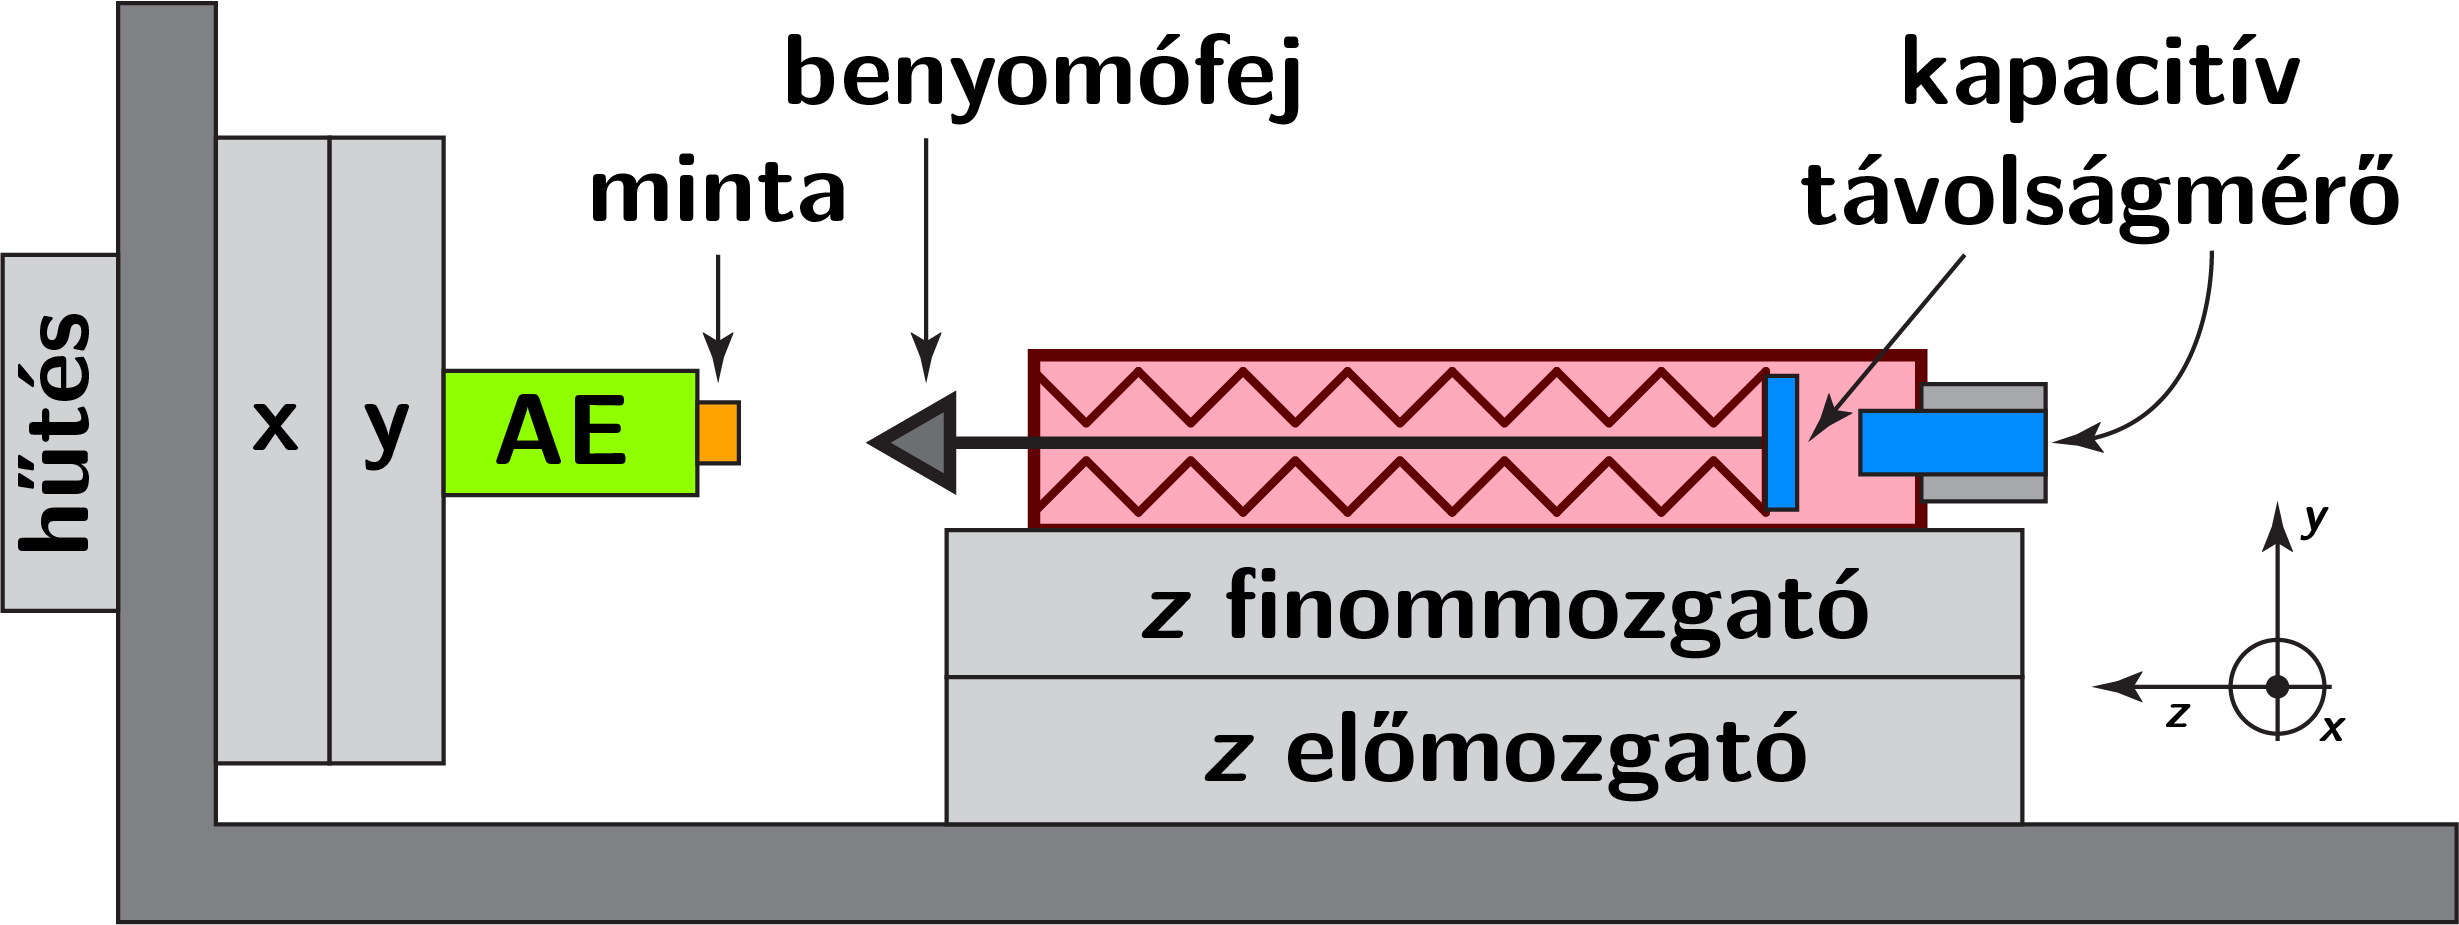
\includegraphics[width=1\textwidth]{figs/vazlat.png} 
\end{frame}


\begin{frame}
\frametitle{[4] Akusztikus jelek a deformációgörbén}
\begin{itemize}
\item PLC instabil anyagon először
\item Diszlokációlavinák vizsgálatára később
\end{itemize}
\centering
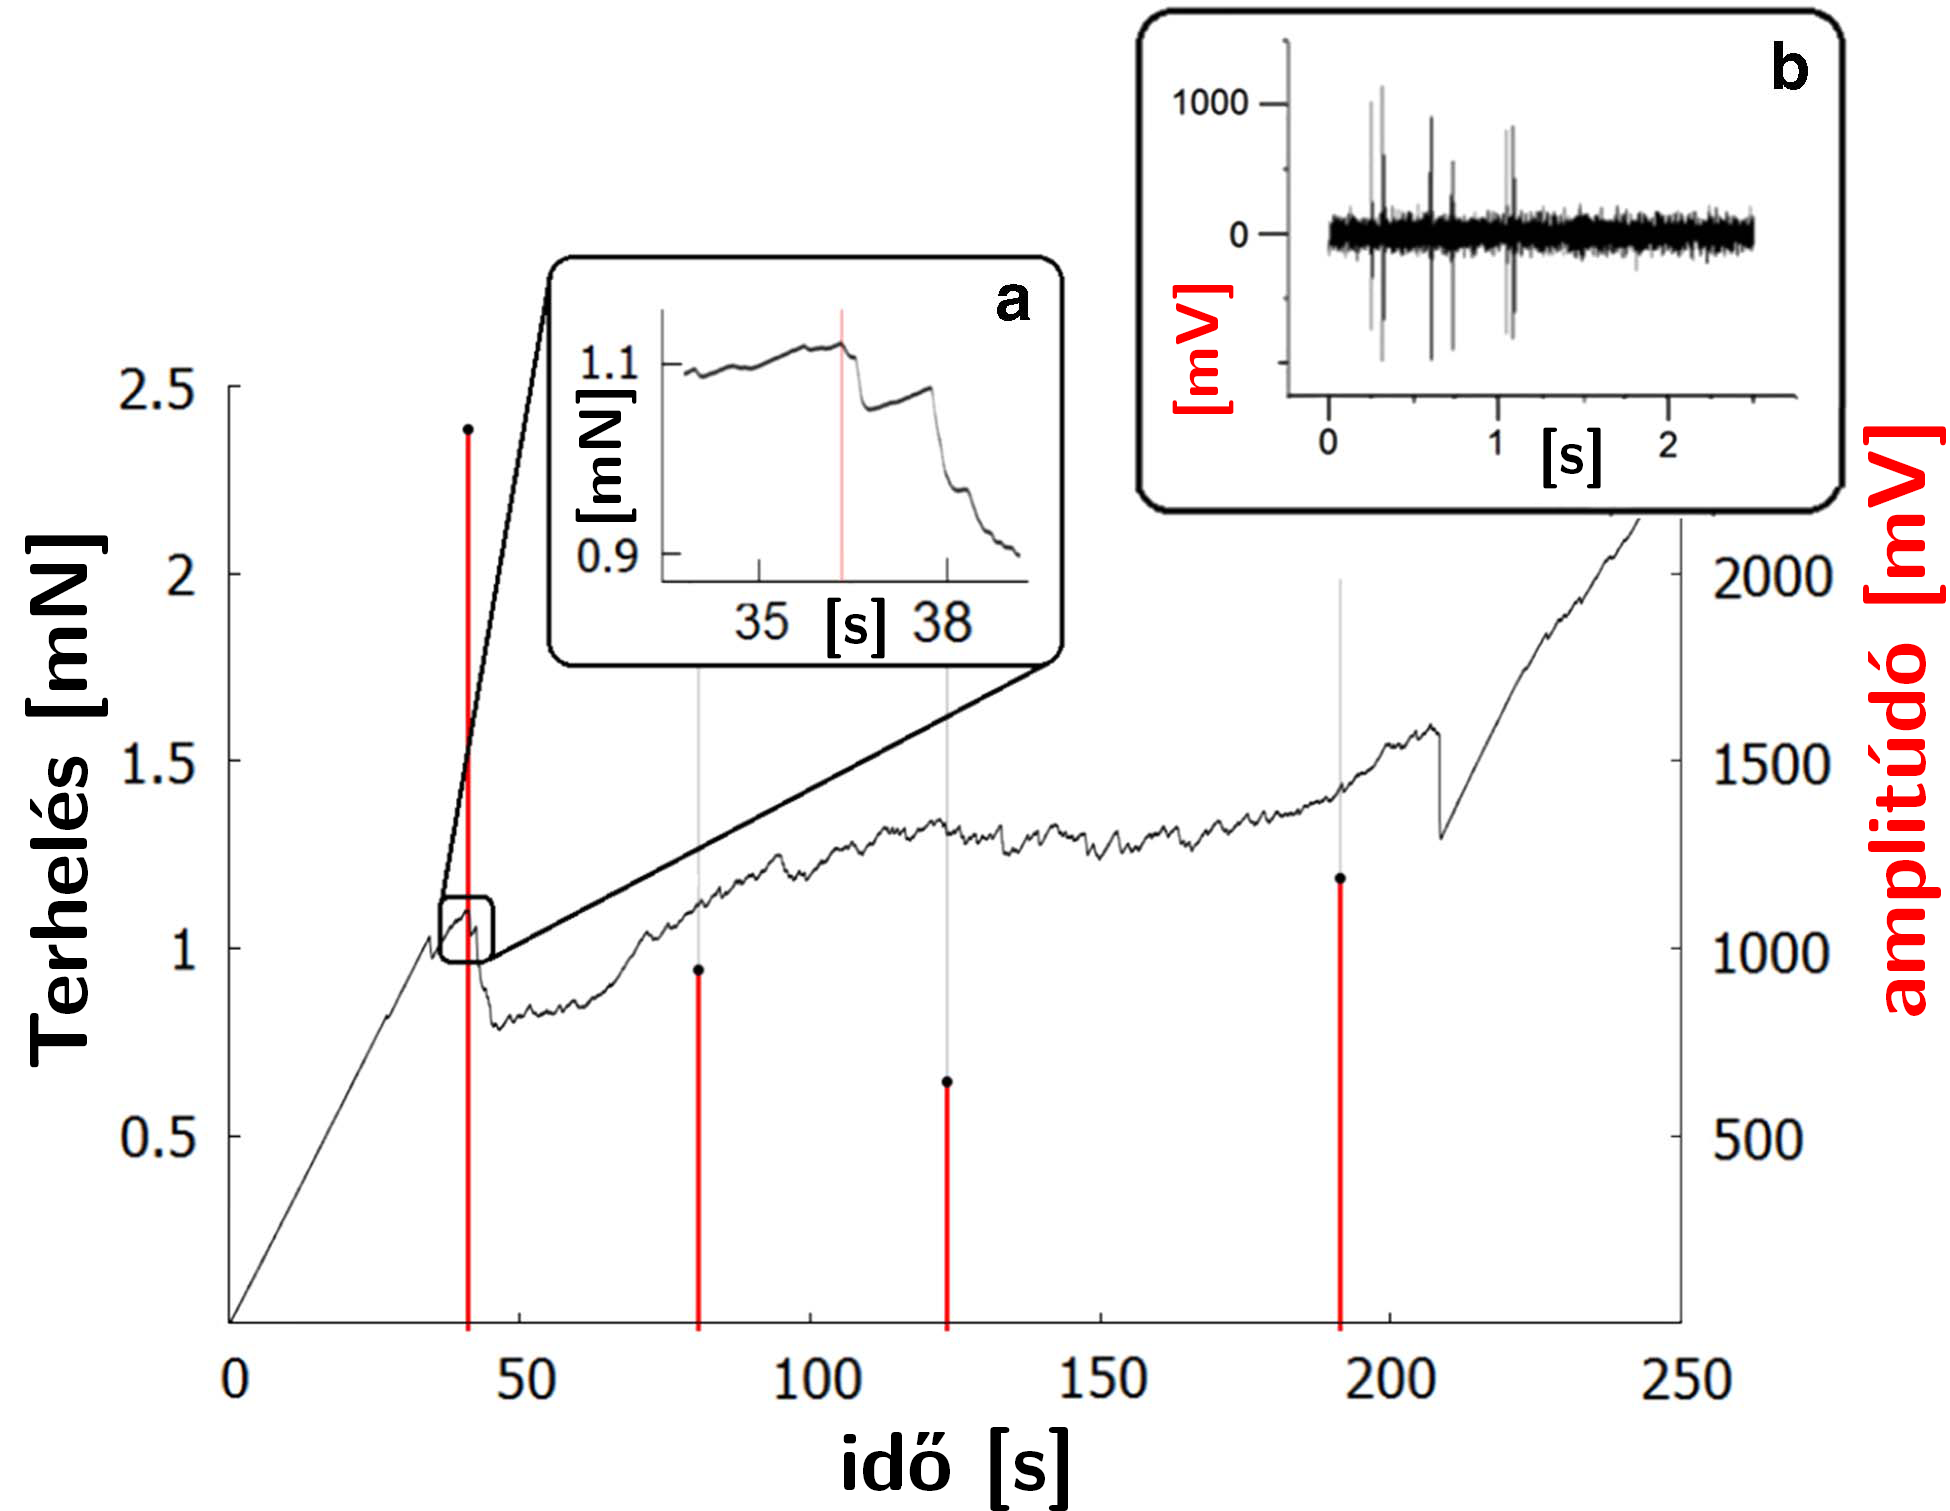
\includegraphics[width=0.7\textwidth]{figs/Micron_Scale_Deformation.png} 
\end{frame}


\begin{frame}
\frametitle{Eredmények}
\begin{itemize}
\item működik a nanoindenter
\item elfér az elektronmikroszkóp kamrájában
\item alkalmas in-situ vizsgálatra
\item akusztikus jeleket is detektál
\end{itemize}
\end{frame}

\begin{frame}
\footnotesize
\begin{itemize}
\item[1] Péter Dusán Ispánovity, Dániel Tüzes, Péter Szabó, Michael
Zaiser, and István Groma. “Role of weakest links and systemsize
scaling in multiscale modeling of stochastic plasticity”.
In: Phys. Rev. B 95 (5 Feb. 2017), p. 054108.
\item[2] Dániel Tüzes, Péter Dusán Ispánovity, and Michael Zaiser.
“Disorder is good for you: the influence of local disorder on
strain localization and ductility of strain softening materials”.
In: International Journal of Fracture 205.2 (June 2017),
pp. 139–150. issn: 1573-2673.
\item[3] Ronghai Wu, Dániel Tüzes, Péter Dusán Ispánovity, István
Groma, Thomas Hochrainer, and Michael Zaiser. “Instability
of dislocation fluxes in a single slip: Deterministic and stochastic
models of dislocation patterning”. In: Phys. Rev. B 98 (5
Aug. 2018), p. 054110.
\item[4] Ádám István Hegyi, Péter Dusán Ispánovity, Michal Knapek,
Dániel Tüzes, Kristián Máthis, František Chmelík, Zoltán Dankházi,
Gábor Varga, and István Groma. “Micron-Scale Deformation:
A Coupled In Situ Study of Strain Bursts and Acoustic
Emission”. In: Microscopy and Microanalysis 23.6 (2017),
pp. 1076–1081.
\end{itemize}
\end{frame}

\begin{frame}
\frametitle{Források, hivatkozások}
\begin{itemize}
\item
The probability distribution of internal stresses in externally loaded 2D dislocation systems; Péter Dusán Ispánovity and István Groma; Published 16 December 2008; IOP
\item
István Groma, Michael Zaiser, and Péter Dusán Ispánovity.
“Dislocation patterning in a two-dimensional continuum theory
of dislocations”. In: Phys. Rev. B 93 (21 June 2016),
p. 214110. doi: 10.1103/PhysRevB.93.214110.
\item
Michael Zaiser and Paolo Moretti. “Fluctuation phenomena
in crystal plasticity—a continuum model”. In: Journal of Statistical
Mechanics: Theory and Experiment 2005.08 (2005),
P08004. doi: 10.1088/1742-5468/2005/08/P08004.
\end{itemize}

\end{frame}


\end{document}

